\setlength{\headheight}{14.93912pt}  % Điều chỉnh chiều cao của header
\addtolength{\topmargin}{-2.93912pt} % Giảm lề trên để bù trừ cho chiều cao header

\pagestyle{fancy} 

\fancyhf{}  % Xóa tất cả các thiết lập mặc định cho header và footer
\fancyhead[L]{Chương 3: Thực nghiệm và đánh giá}  % Header bên trái (L)
\fancyhead[R]{Bùi Minh Thành}  % Header bên phải (R)

\fancyfoot[C]{\thepage}  % Đặt số trang vào footer ở giữa (C)

\chapter[Thực nghiệm và đánh giá]{\centering Thực nghiệm và đánh giá}

\section{Các bước thực hiện:}

\subsection{Lưu đồ thể hiện các bước trong bài code:}

\begin{figure}[h]
    \centering
    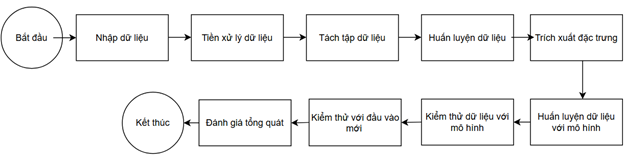
\includegraphics[width=1\textwidth]{img/docspics/02_progress.png}
\end{figure}

\subsection{Các thư viện được sử dụng trong code:}

\begin{enumerate}
    \item NumPy: là thư viện cơ bản cho tính toán khoa học trong Python, cung cấp cấu trúc mảng đa chiều hiệu quả và các hàm toán học mạnh mẽ.
    \item Pandas: là thư viện phân tích dữ liệu mạnh mẽ, cung cấp cấu trúc DataFrame cho phép lưu trữ và thao tác dữ liệu dạng bảng dễ dàng.
    \item Scikit-learn (sklearn): là thư viện hàng đầu cho học máy, cung cấp các thuật toán phân loại, hồi quy, phân cụm và các công cụ đánh giá mô hình.
    \item Seaborn: là thư viện trực quan hóa dữ liệu dựa trên matplotlib, giúp tạo ra các biểu đồ thống kê đẹp mắt và dễ hiểu.
    \item Matplotlib: là thư viện cơ bản để tạo biểu đồ trong Python, hỗ trợ nhiều loại biểu đồ và cho phép tùy chỉnh cao.
    \item SciPy là thư viện cho tính toán khoa học và kỹ thuật, cung cấp các công cụ cho đại số tuyến tính, tối ưu hóa, tích phân và vi phân.
    \item Langdetect: là thư viện xác định ngôn ngữ của đoạn văn bản, hỗ trợ nhiều ngôn ngữ và dễ sử dụng.
\end{enumerate}

\subsection{Giải thích chi tiết từng bước (character):}

\textbf{Bước 1: Nhập dữ liệu:}
\begin{figure}[H]
    \centering
    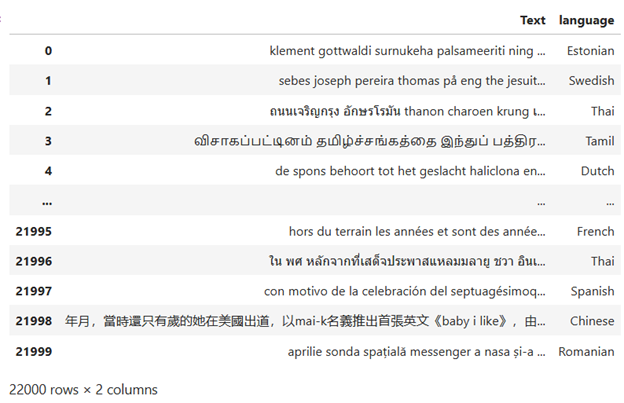
\includegraphics[width=1\textwidth]{img/docspics/Picture2.png}
\end{figure}
\textbf{Bước 2: Tiền xử lý dữ liệu:}
\begin{figure}[H]
    \centering
    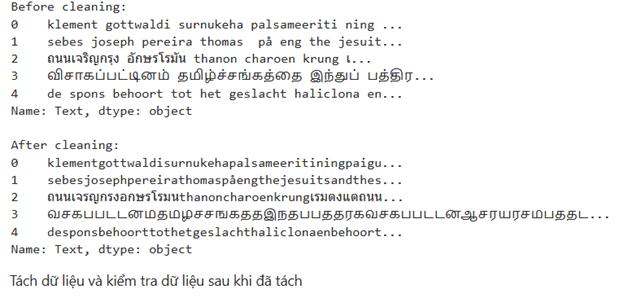
\includegraphics[width=1\textwidth]{img/docspics/Picture3.png}
\end{figure}
\clearpage
\textbf{Bước 3: Tách dữ liệu:}
\begin{figure}[H]
    \centering
    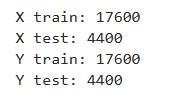
\includegraphics[width=0.3\textwidth]{img/docspics/Picture4.png}
\end{figure}
\textbf{Bước 4: Trích xuất đặc trưng:}
\begin{itemize}
    \item Uni-grams: 
    \begin{figure}[H]
    \centering
    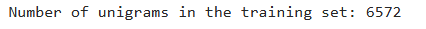
\includegraphics[width=0.8\textwidth]{img/docspics/Picture5.png}
\end{figure}
    \item Bi-grams:
    \begin{figure}[H]
    \centering
    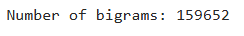
\includegraphics[width=0.5\textwidth]{img/docspics/Picture6.png}
\end{figure}
    \item Cả Uni-grams và Bi-grams (1\% Mixture):
    \begin{figure}[H]
    \centering
    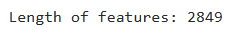
\includegraphics[width=0.5\textwidth]{img/docspics/Picture7.png}
\end{figure}
    \end{itemize}
    
\textbf{Bước 5: Xây dựng từ điển đặc trưng (tần xuất xuất hiện):}
\begin{figure}[H]
    \centering
    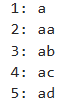
\includegraphics[width=0.1\textwidth]{img/docspics/Picture8.png}
\end{figure}
\clearpage
\textbf{Bước 6: Huấn luyện dữ liệu:}
\begin{itemize}
    \item Uni-Grams:
    \begin{figure}[H]
    \centering
    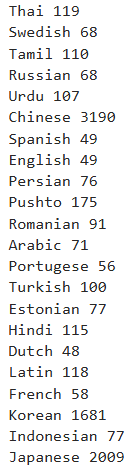
\includegraphics[width=0.2\textwidth]{img/docspics/Picture9.png}
\end{figure}
    \item Bi-Grams (1\%):
    \begin{figure}[H]
    \centering
    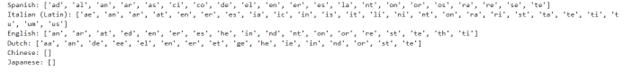
\includegraphics[width=1\textwidth]{img/docspics/Picture12.png}
\end{figure}
\clearpage
    \item Mixture (Top 1\%):
    \begin{figure}[H]
    \centering
    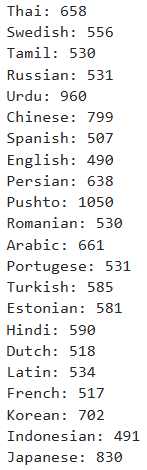
\includegraphics[width=0.2\textwidth]{img/docspics/Picture13.png}
\end{figure}
    \item Mixture (Top 50):
    \begin{figure}[H]
    \centering
    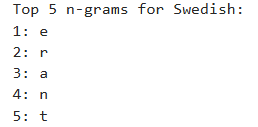
\includegraphics[width=0.5\textwidth]{img/docspics/Picture14.png}
\end{figure}
\end{itemize}
\clearpage
\textbf{Bước 7: Kiểm thử dữ liệu với mô hình:}

\begin{itemize}
    \item Ma trận có được:
    \begin{itemize}
        \item Uni-Grams:
        \begin{figure}[H]
    \centering
    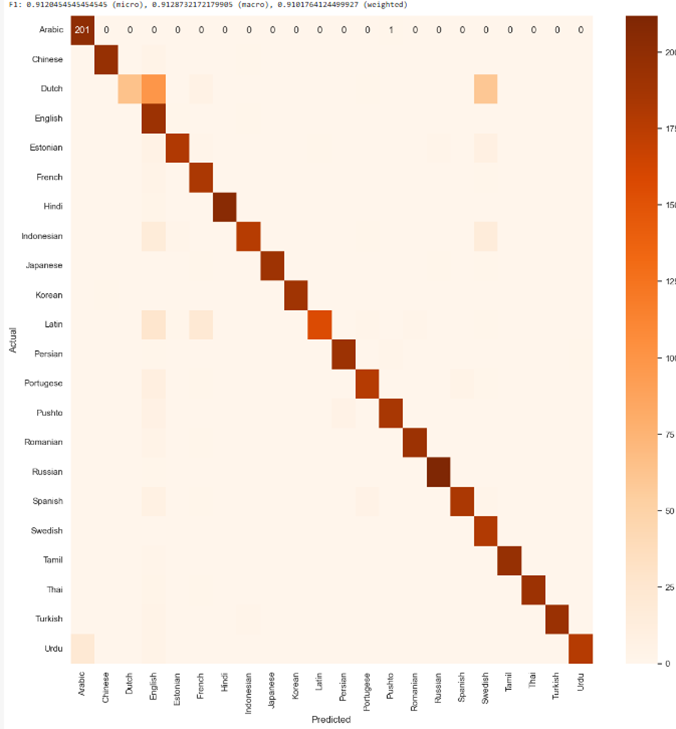
\includegraphics[width=1\textwidth]{img/docspics/Picture15.png}
\end{figure}
\clearpage
        \item Bi-Grams:
        \begin{figure}[H]
    \centering
    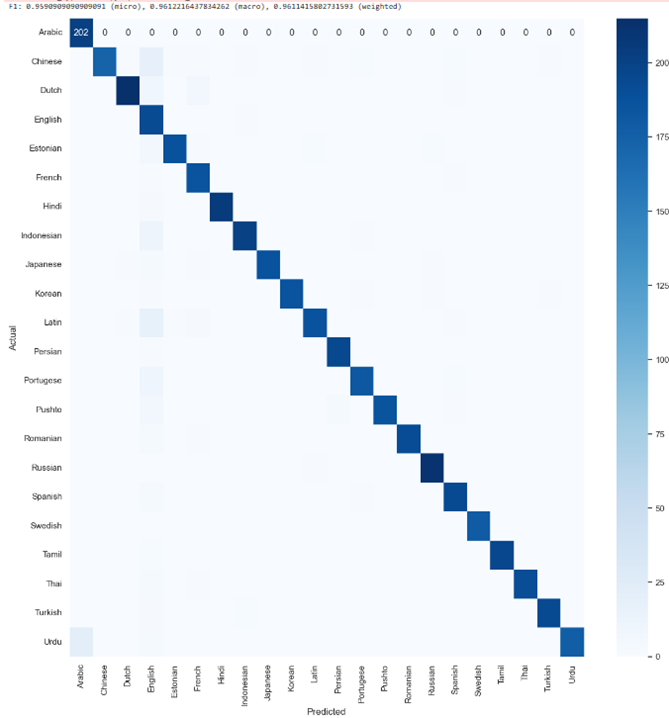
\includegraphics[width=1\textwidth]{img/docspics/Picture16.png}
\end{figure}
\clearpage
        \item Mixture (Top 1\%):
        \begin{figure}[H]
    \centering
    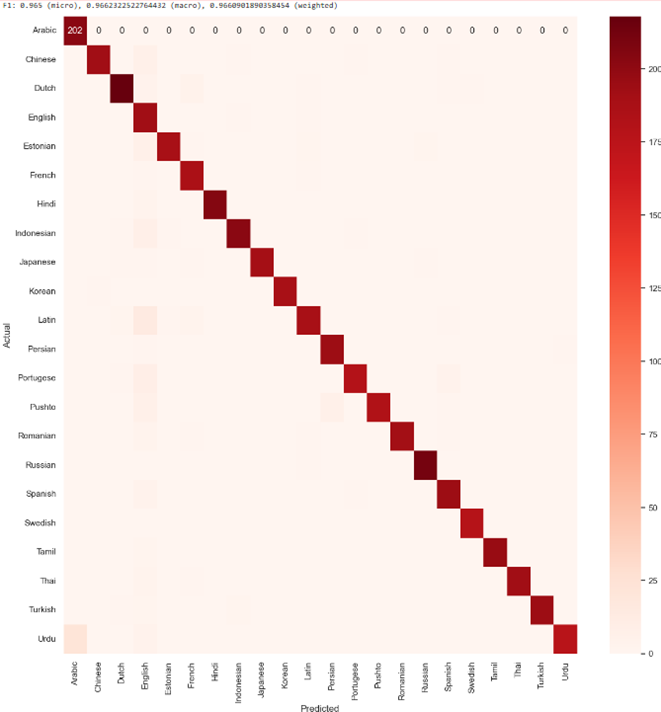
\includegraphics[width=1\textwidth]{img/docspics/Picture17.png}
\end{figure}
\clearpage
        \item Mixture (Top 50):
        \begin{figure}[H]
    \centering
    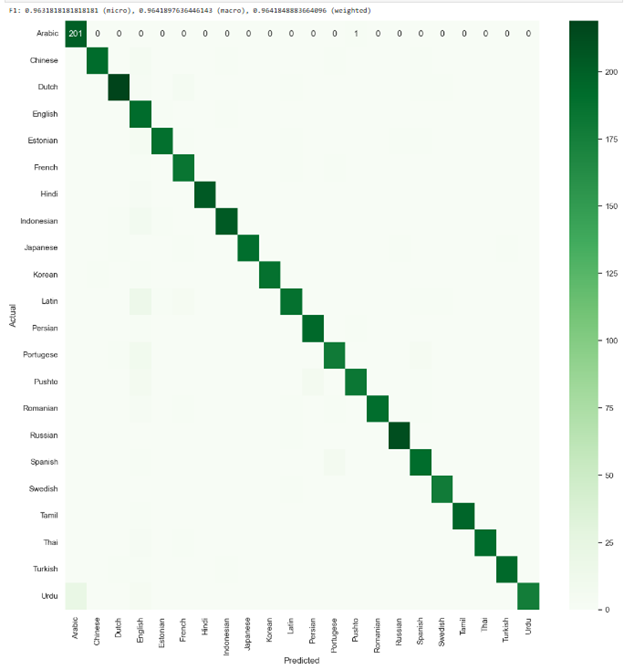
\includegraphics[width=1\textwidth]{img/docspics/Picture18.png}
\end{figure}
    \end{itemize}
\end{itemize}

\textbf{Bước 8: Kiểm thử mô hình đã huấn luyện với dữ liệu đầu vào mới:}

\textbf{Bước 9: Đánh giá tổng quát:}
\begin{itemize}
    \item Các trường hợp dự đoán sai của máy:
    \begin{figure}[H]
    \centering
    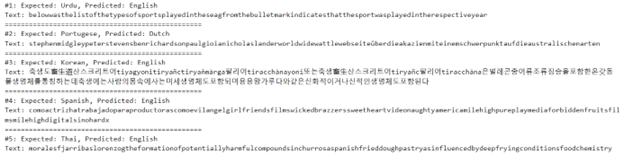
\includegraphics[width=1\textwidth]{img/docspics/Picture19.png}
\end{figure}
    \item Các trường hợp dự đoán đúng của máy:
    \begin{figure}[H]
    \centering
    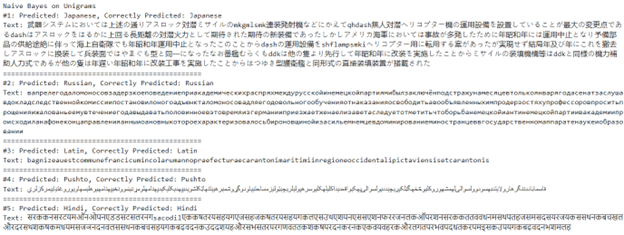
\includegraphics[width=1\textwidth]{img/docspics/Picture20.png}
\end{figure}
    \item Kiểm tra độ chính xác của từng bộ huấn luyện:
    \begin{itemize}
        \item Uni-Grams:
        \begin{figure}[H]
    \centering
    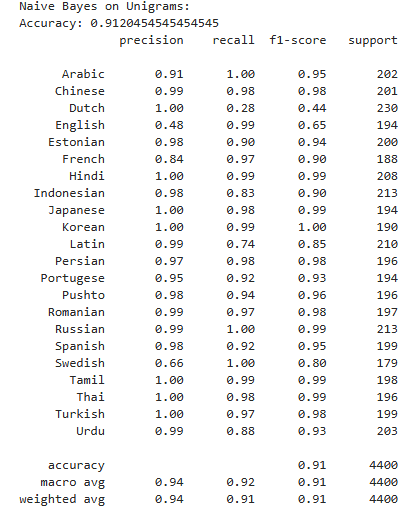
\includegraphics[width=0.7\textwidth]{img/docspics/Picture21.png}
\end{figure}
\clearpage
        \item Bi-Grams:
        \begin{figure}[H]
    \centering
    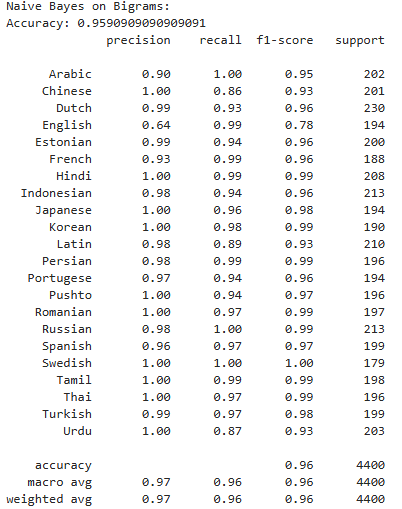
\includegraphics[width=0.7\textwidth]{img/docspics/Picture22.png}
\end{figure}
\clearpage
        \item Mixture (Top 50):
        \begin{figure}[H]
    \centering
    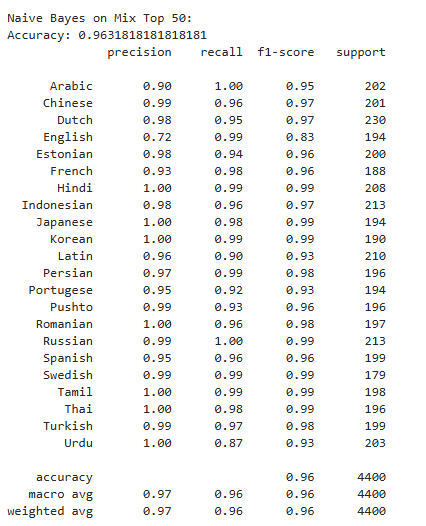
\includegraphics[width=0.7\textwidth]{img/docspics/Picture23.png}
\end{figure}
\clearpage
        \item Mixture (Top 1\%):
        \begin{figure}[H]
    \centering
    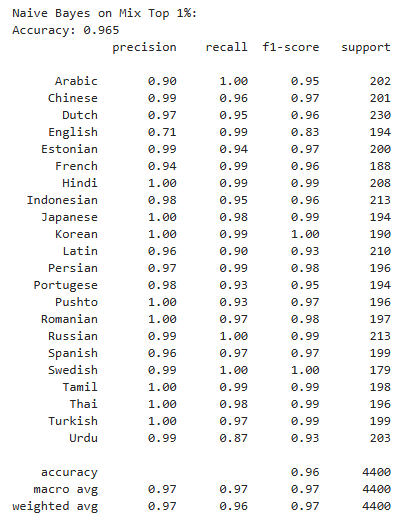
\includegraphics[width=0.7\textwidth]{img/docspics/Picture24.png}
\end{figure}
    \end{itemize}
\end{itemize}
\clearpage
\subsection{Giải thích chi tiết từng bước (word):}

\textbf{Bước 1: Nhập dữ liệu:}
\begin{figure}[H]
    \centering
    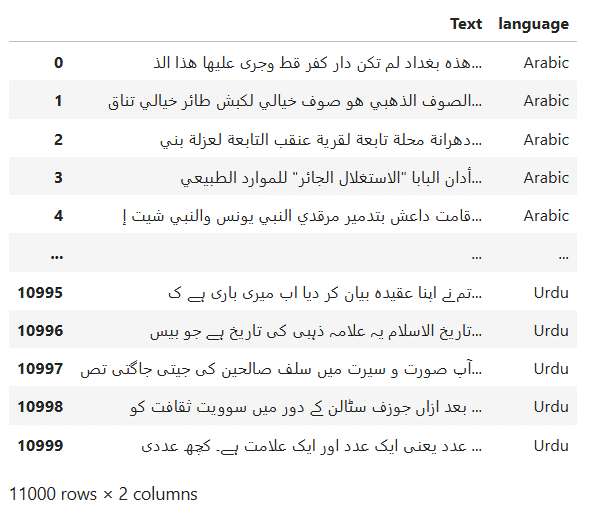
\includegraphics[width=0.8\textwidth]{img/docspics/Picture25.png}
\end{figure}
\textbf{Bước 2: Tiền xử lý dữ liệu:}
\begin{figure}[H]
    \centering
    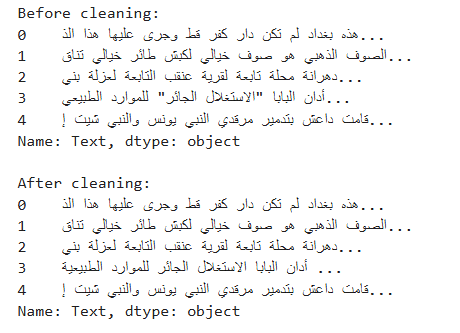
\includegraphics[width=0.8\textwidth]{img/docspics/Picture26.png}
\end{figure}
\clearpage
\textbf{Bước 3: Tách dữ liệu:}
\begin{figure}[H]
    \centering
    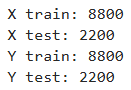
\includegraphics[width=0.3\textwidth]{img/docspics/Picture27.png}
\end{figure}
\textbf{Bước 4: Trích xuất đặc trưng:}
\begin{itemize}
    \item Uni-grams: 
    \begin{figure}[H]
    \centering
    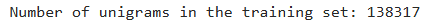
\includegraphics[width=0.8\textwidth]{img/docspics/Picture28.png}
\end{figure}
    \item Bi-grams:
    \begin{figure}[H]
    \centering
    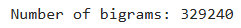
\includegraphics[width=0.5\textwidth]{img/docspics/Picture29.png}
\end{figure}
    \item Cả Uni-grams và Bi-grams (1\% Mixture):
    \begin{figure}[H]
    \centering
    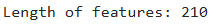
\includegraphics[width=0.5\textwidth]{img/docspics/Picture30.png}
\end{figure}
    \end{itemize}
    
\textbf{Bước 5: Xây dựng từ điển đặc trưng (tần xuất xuất hiện):}
\begin{figure}[H]
    \centering
    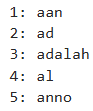
\includegraphics[width=0.2 \textwidth]{img/docspics/Picture31.png}
\end{figure}
\clearpage
\textbf{Bước 6: Huấn luyện dữ liệu:}

\begin{itemize}
    \item Uni-Grams:
    \begin{figure}[H]
    \centering
    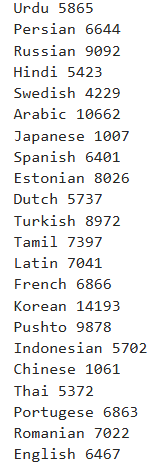
\includegraphics[width=0.3\textwidth]{img/docspics/Picture32.png}
\end{figure}
    \item Bi-Grams (1\%):
    \begin{figure}[H]
    \centering
    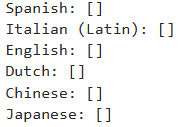
\includegraphics[width=0.3\textwidth]{img/docspics/Picture33.png}
\end{figure}
\clearpage
    \item Mixture (Top 1\%):
    \begin{figure}[H]
    \centering
    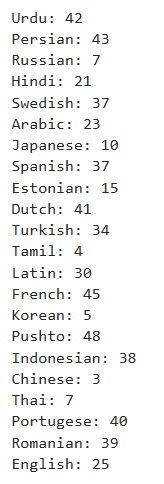
\includegraphics[width=0.3\textwidth]{img/docspics/Picture34.png}
\end{figure}
    \item Mixture (Top 50):
    \begin{figure}[H]
    \centering
    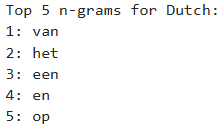
\includegraphics[width=0.4\textwidth]{img/docspics/Picture35.png}
\end{figure}
\end{itemize}
\clearpage
\textbf{Bước 7: Kiểm thử dữ liệu với mô hình:}

\begin{itemize}
    \item Ma trận có được:
    \begin{itemize}
        \item Uni-Grams:
        \begin{figure}[H]
    \centering
    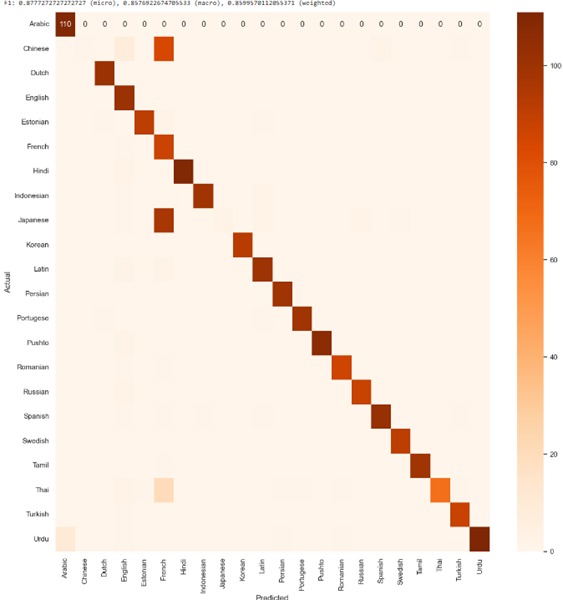
\includegraphics[width=1\textwidth]{img/docspics/Picture36.png}
\end{figure}
\clearpage
        \item Bi-Grams:
        \begin{figure}[H]
    \centering
    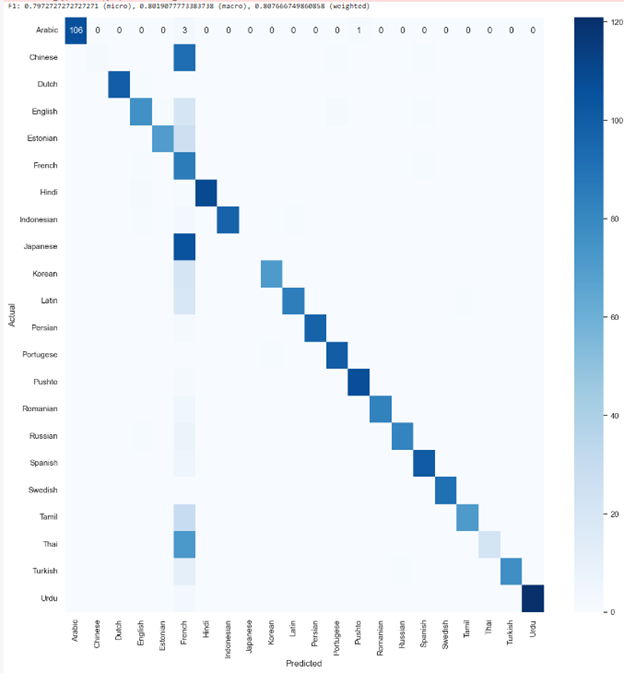
\includegraphics[width=1\textwidth]{img/docspics/Picture37.png}
\end{figure}
\clearpage
        \item Mixture (Top 1\%):
        \begin{figure}[H]
    \centering
    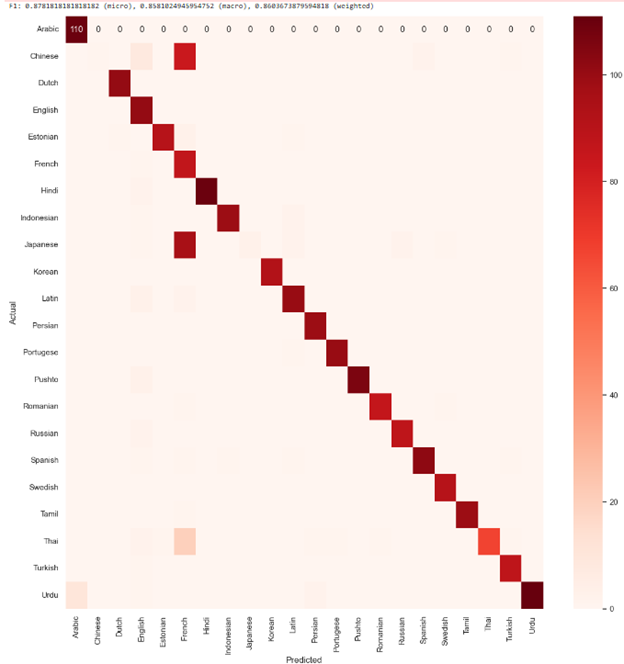
\includegraphics[width=1\textwidth]{img/docspics/Picture38.png}
\end{figure}
\clearpage
        \item Mixture (Top 50):
        \begin{figure}[H]
    \centering
    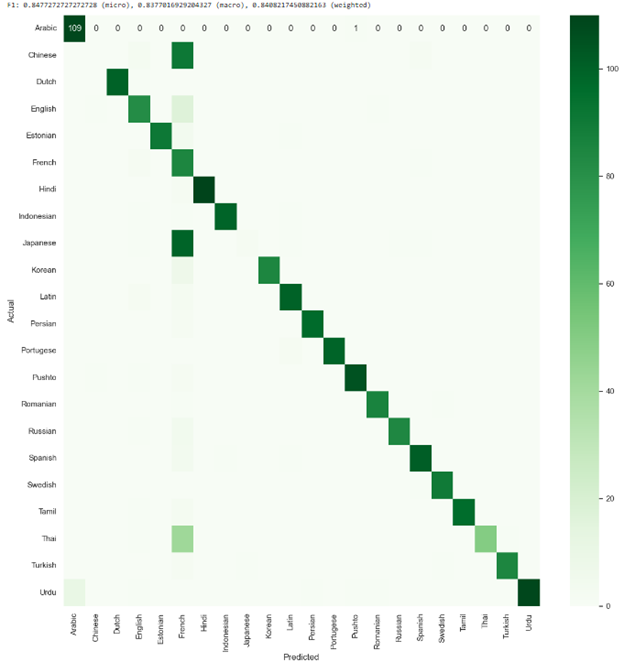
\includegraphics[width=1\textwidth]{img/docspics/Picture39.png}
\end{figure}
    \end{itemize}
\end{itemize}
\clearpage
\textbf{Bước 8: Kiểm thử mô hình đã huấn luyện với dữ liệu đầu vào mới:}

\textbf{Bước 9: Đánh giá tổng quát:}
\begin{itemize}
    \item Các trường hợp dự đoán sai của máy:
    \begin{figure}[H]
    \centering
    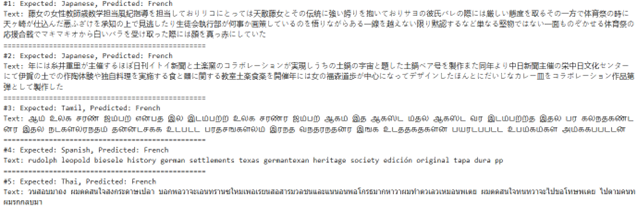
\includegraphics[width=1\textwidth]{img/docspics/Picture40.png}
\end{figure}
    \item Các trường hợp dự đoán đúng của máy:
    \begin{figure}[H]
    \centering
    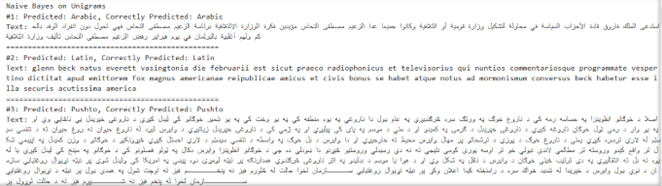
\includegraphics[width=1\textwidth]{img/docspics/Picture41.png}
\end{figure}
\clearpage
    \item Kiểm tra độ chính xác của từng bộ huấn luyện:
    \begin{itemize}
        \item Uni-Grams:
        \begin{figure}[H]
    \centering
    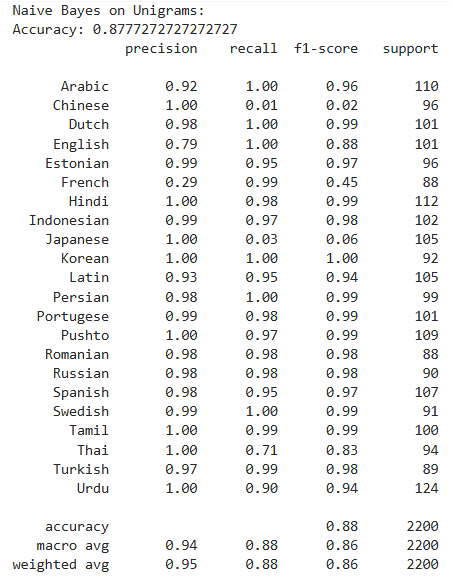
\includegraphics[width=0.7\textwidth]{img/docspics/Picture42.png}
\end{figure}
\clearpage
        \item Bi-Grams:
        \begin{figure}[H]
    \centering
    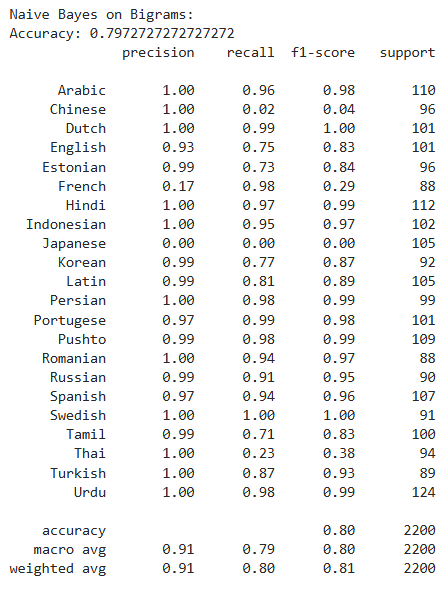
\includegraphics[width=0.7\textwidth]{img/docspics/Picture43.png}
\end{figure}
\clearpage
        \item Mixture (Top 50):
        \begin{figure}[H]
    \centering
    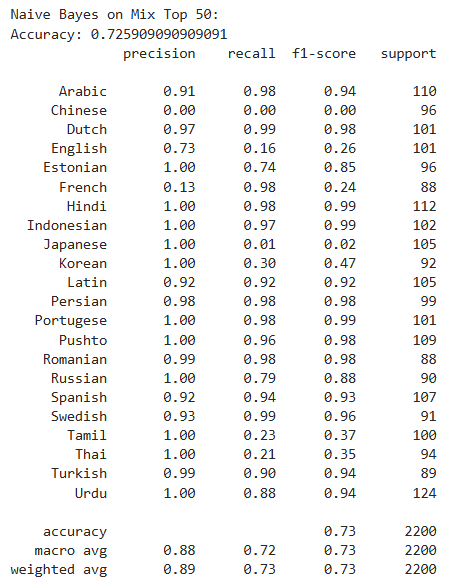
\includegraphics[width=0.7\textwidth]{img/docspics/Picture44.png}
\end{figure}
\clearpage
        \item Mixture (Top 1\%):
        \begin{figure}[H]
    \centering
    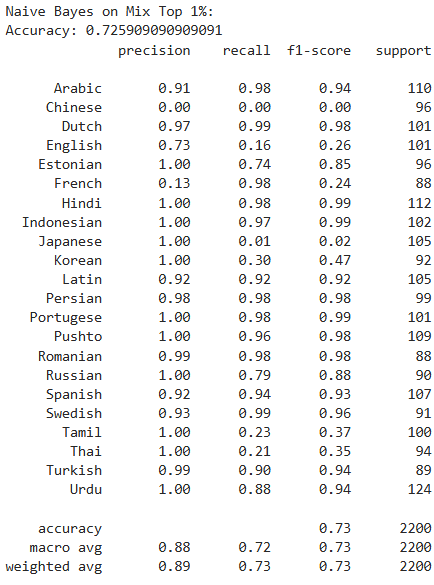
\includegraphics[width=0.7\textwidth]{img/docspics/Picture45.png}
\end{figure}
\end{itemize}

\end{itemize}
\clearpage
\subsection{Giới thiệu về các thuật toán khác được sử dụng trong bài:}

\begin{enumerate}
    \item K Nearest Neighbour:
    \begin{itemize}
        \item K Nearest Neighbour (KNN) là một thuật toán đơn giản và hiệu quả trong học máy, được sử dụng cho cả phân loại và hồi quy. Thuật toán hoạt động bằng cách tìm k điểm dữ liệu gần nhất trong không gian đặc trưng và dự đoán giá trị dựa trên các điểm đó.
        \item KNN không yêu cầu giai đoạn huấn luyện. Thay vào đó, nó lưu trữ toàn bộ tập dữ liệu huấn luyện và thực hiện tính toán tại thời điểm dự đoán. Điều này làm cho KNN đơn giản nhưng có thể chậm nếu tập dữ liệu lớn.
    \end{itemize}
    \item (Ordinary) Least Squares:
    \begin{itemize}
        \item Ordinary Least Squares (OLS) là một phương pháp thống kê để ước lượng các tham số trong mô hình hồi quy tuyến tính. Nó tìm các tham số sao cho tổng bình phương sai số giữa giá trị dự đoán và giá trị thực là nhỏ nhất.
        \item OLS đơn giản và dễ triển khai. Nó cung cấp các ước lượng hiệu quả và không chệch trong điều kiện nhiễu có phân phối chuẩn.
    \end{itemize}
    \item Kolmogorov Smirnov Test:
    \begin{itemize}
        \item Kolmogorov-Smirnov Test (KS Test) là một kiểm định phi tham số dùng để so sánh hai phân phối xác suất hoặc một phân phối với một phân phối tham chiếu. Nó dựa trên sự khác biệt lớn nhất giữa hai hàm phân phối tích lũy (CDF).
        \item KS Test không phụ thuộc vào dạng phân phối của dữ liệu, làm cho nó rất linh hoạt. Nó có thể được sử dụng cho cả dữ liệu liên tục và dữ liệu rời rạc.
    \end{itemize}
    \item Lang Detect:
    \begin{itemize}
        \item Lang Detect là một thư viện dùng để phát hiện ngôn ngữ của một đoạn văn bản dựa trên mô hình học máy. Nó sử dụng các kỹ thuật như Naive Bayes hoặc n-gram để xác định ngôn ngữ.
        \item Lang Detect rất hiệu quả và hỗ trợ nhiều ngôn ngữ khác nhau. Nó dễ sử dụng và tích hợp vào các ứng dụng xử lý ngôn ngữ tự nhiên.
    \end{itemize}

\end{enumerate}
\clearpage
\section{Kết quả thực nghiệm:}

\subsection{Thực nghiệm trên 10 từ (character):}

\begin{enumerate}
    \item NB trên Unigrams:
    \begin{figure}[H]
    \centering
    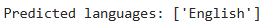
\includegraphics[width=0.7\textwidth]{img/docspics/Picture46.png}
\end{figure}
    \item NB trên Bigrams:
    \begin{figure}[H]
    \centering
    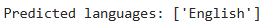
\includegraphics[width=0.7\textwidth]{img/docspics/Picture47.png}
\end{figure}
    \item NB trên Mix Top 50:
    \begin{figure}[H]
    \centering
    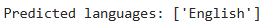
\includegraphics[width=0.7\textwidth]{img/docspics/Picture48.png}
\end{figure}
    \item NB trên Mix Top 1\%:
    \begin{figure}[H]
    \centering
    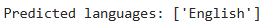
\includegraphics[width=0.7\textwidth]{img/docspics/Picture49.png}
\end{figure}
    \item KNN trên Mix Top 50:
    \begin{figure}[H]
    \centering
    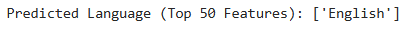
\includegraphics[width=0.7\textwidth]{img/docspics/Picture50.png}
\end{figure}
    \item OLS trên Mix Top 50:
    \begin{figure}[H]
    \centering
    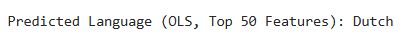
\includegraphics[width=0.7\textwidth]{img/docspics/Picture51.png}
\end{figure}
    \item Langdetect:
    \begin{figure}[H]
    \centering
    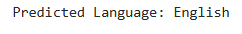
\includegraphics[width=0.7\textwidth]{img/docspics/Picture52.png}
\end{figure}
    \item KS trên Mix Top 50:
    \begin{figure}[H]
    \centering
    \includegraphics[width=0.7\textwidth]{img/docspics/Picture53.png}
\end{figure}
\end{enumerate}

\subsection{Thực nghiệm trên 50 từ (character):}

\begin{enumerate}
    \item NB trên Unigrams:
    \begin{figure}[H]
    \centering
    \includegraphics[width=0.7\textwidth]{img/docspics/Picture54.png}
\end{figure}
    \item NB trên Bigrams:
    \begin{figure}[H]
    \centering
    \includegraphics[width=0.7\textwidth]{img/docspics/Picture55.png}
\end{figure}
    \item NB trên Mix Top 50:
    \begin{figure}[H]
    \centering
    \includegraphics[width=0.7\textwidth]{img/docspics/Picture56.png}
\end{figure}
    \item NB trên Mix Top 1\%:
    \begin{figure}[H]
    \centering
    \includegraphics[width=0.7\textwidth]{img/docspics/Picture57.png}
\end{figure}
    \item KNN trên Mix Top 50:
    \begin{figure}[H]
    \centering
    \includegraphics[width=0.7\textwidth]{img/docspics/Picture58.png}
\end{figure}
    \item OLS trên Mix Top 50:
    \begin{figure}[H]
    \centering
    \includegraphics[width=0.7\textwidth]{img/docspics/Picture59.png}
\end{figure}
    \item Langdetect:
    \begin{figure}[H]
    \centering
    \includegraphics[width=0.7\textwidth]{img/docspics/Picture60.png}
\end{figure}
    \item KS trên Mix Top 50:
    \begin{figure}[H]
    \centering
    \includegraphics[width=0.7\textwidth]{img/docspics/Picture61.png}
\end{figure}
\end{enumerate}

\subsection{Thực nghiệm trên 100 từ (character):}

\begin{enumerate}
    \item NB trên Unigrams:
    \begin{figure}[H]
    \centering
    \includegraphics[width=0.7\textwidth]{img/docspics/Picture62.png}
\end{figure}
    \item NB trên Bigrams:
    \begin{figure}[H]
    \centering
    \includegraphics[width=0.7\textwidth]{img/docspics/Picture63.png}
\end{figure}
    \item NB trên Mix Top 50:
    \begin{figure}[H]
    \centering
    \includegraphics[width=0.7\textwidth]{img/docspics/Picture64.png}
\end{figure}
    \item NB trên Mix Top 11\%:
    \begin{figure}[H]
    \centering
    \includegraphics[width=0.7\textwidth]{img/docspics/Picture65.png}
\end{figure}
    \item KNN trên Mix Top 50:
    \begin{figure}[H]
    \centering
    \includegraphics[width=0.7\textwidth]{img/docspics/Picture66.png}
\end{figure}
    \item OLS trên Mix Top 50:
    \begin{figure}[H]
    \centering
    \includegraphics[width=0.7\textwidth]{img/docspics/Picture67.png}
\end{figure}
    \item Langdetect:
    \begin{figure}[H]
    \centering
    \includegraphics[width=0.7\textwidth]{img/docspics/Picture68.png}
\end{figure}
    \item KS trên Mix Top 50:
    \begin{figure}[H]
    \centering
    \includegraphics[width=0.7\textwidth]{img/docspics/Picture69.png}
\end{figure}
\end{enumerate}

\subsection{Thực nghiệm trên 10 từ (word):}

\begin{enumerate}
    \item NB trên Unigrams:
    \begin{figure}[H]
    \centering
    \includegraphics[width=0.7\textwidth]{img/docspics/Picture70.png}
\end{figure}
    \item NB trên Bigrams:
    \begin{figure}[H]
    \centering
    \includegraphics[width=0.7\textwidth]{img/docspics/Picture71.png}
\end{figure}
    \item NB trên Mix Top 50:
    \begin{figure}[H]
    \centering
    \includegraphics[width=0.7\textwidth]{img/docspics/Picture72.png}
\end{figure}
    \item NB trên Mix Top 1\%:
    \begin{figure}[H]
    \centering
    \includegraphics[width=0.7\textwidth]{img/docspics/Picture73.png}
\end{figure}
    \item KNN trên Mix Top 50:
    \begin{figure}[H]
    \centering
    \includegraphics[width=0.7\textwidth]{img/docspics/Picture74.png}
\end{figure}
    \item OLS trên Mix Top 50:
    \begin{figure}[H]
    \centering
    \includegraphics[width=0.7\textwidth]{img/docspics/Picture75.png}
\end{figure}
    \item Langdetect:
    \begin{figure}[H]
    \centering
    \includegraphics[width=0.7\textwidth]{img/docspics/Picture76.png}
\end{figure}
    \item KS trên Mix Top 50:
    \begin{figure}[H]
    \centering
    \includegraphics[width=0.7\textwidth]{img/docspics/Picture77.png}
\end{figure}
\end{enumerate}

\subsection{Thực nghiệm trên 50 từ (word):}

\begin{enumerate}
    \item NB trên Unigrams:
    \begin{figure}[H]
    \centering
    \includegraphics[width=0.7\textwidth]{img/docspics/Picture78.png}
\end{figure}
    \item NB trên Bigrams:
    \begin{figure}[H]
    \centering
    \includegraphics[width=0.7\textwidth]{img/docspics/Picture79.png}
\end{figure}
    \item NB trên Mix Top 50:
    \begin{figure}[H]
    \centering
    \includegraphics[width=0.7\textwidth]{img/docspics/Picture80.png}
\end{figure}
    \item NB trên Mix Top 1\%:
    \begin{figure}[H]
    \centering
    \includegraphics[width=0.7\textwidth]{img/docspics/Picture81.png}
\end{figure}
    \item KNN trên Mix Top 50:
    \begin{figure}[H]
    \centering
    \includegraphics[width=0.7\textwidth]{img/docspics/Picture82.png}
\end{figure}
    \item OLS trên Mix Top 50:
    \begin{figure}[H]
    \centering
    \includegraphics[width=0.7\textwidth]{img/docspics/Picture83.png}
\end{figure}
    \item Langdetect:
    \begin{figure}[H]
    \centering
    \includegraphics[width=0.7\textwidth]{img/docspics/Picture84.png}
\end{figure}
    \item KS trên Mix Top 50:
    \begin{figure}[H]
    \centering
    \includegraphics[width=0.7\textwidth]{img/docspics/Picture85.png}
\end{figure}
\end{enumerate}

\subsection{Thực nghiệm trên 100 từ (word):}

\begin{enumerate}
    \item NB trên Unigrams:
    \begin{figure}[H]
    \centering
    \includegraphics[width=0.7\textwidth]{img/docspics/Picture86.png}
\end{figure}
    \item NB trên Bigrams:
    \begin{figure}[H]
    \centering
    \includegraphics[width=0.7\textwidth]{img/docspics/Picture87.png}
\end{figure}
    \item NB trên Mix Top 50:
    \begin{figure}[H]
    \centering
    \includegraphics[width=0.7\textwidth]{img/docspics/Picture88.png}
\end{figure}
    \item NB trên Mix Top 0.7\%:
    \begin{figure}[H]
    \centering
    \includegraphics[width=0.7\textwidth]{img/docspics/Picture89.png}
\end{figure}
    \item KNN trên Mix Top 50:
    \begin{figure}[H]
    \centering
    \includegraphics[width=0.7\textwidth]{img/docspics/Picture90.png}
\end{figure}
    \item OLS trên Mix Top 50:
    \begin{figure}[H]
    \centering
    \includegraphics[width=0.7\textwidth]{img/docspics/Picture91.png}
\end{figure}
    \item Langdetect:
    \begin{figure}[H]
    \centering
    \includegraphics[width=0.7\textwidth]{img/docspics/Picture92.png}
\end{figure}
    \item KS trên Mix Top 50:
    \begin{figure}[H]
    \centering
    \includegraphics[width=0.7\textwidth]{img/docspics/Picture93.png}
\end{figure}
\end{enumerate}

\section{Đánh giá tổng quát về thuật toán:}

\subsection{Đánh giá riêng về thuật toán chính được sử dụng:}

\begin{itemize}
    \item Dễ hiểu: Thuật toán Naive Bayes (MNB) có cơ sở lý thuyết đơn giản và dễ dàng giải thích, giúp người dùng mới có thể nhanh chóng nắm bắt và áp dụng.
    \item Dễ triển khai: Với các thư viện hỗ trợ mạnh mẽ trong Python, việc triển khai MNB trở nên dễ dàng và không đòi hỏi nhiều công sức.
    \item Tập dữ liệu nhỏ: MNB thể hiện hiệu quả tính toán cao khi làm việc với các tập dữ liệu nhỏ, đảm bảo tốc độ xử lý nhanh và kết quả chính xác.
    \item Tập dữ liệu lớn: Khi áp dụng cho các tập dữ liệu lớn, hiệu suất của MNB không những không giảm mà còn được cải thiện đáng kể, nhờ vào khả năng xử lý và học hỏi từ nhiều dữ liệu.
\end{itemize}

\subsection{So sánh với các thuật toán khác:}

\begin{itemize}

    \item Độ chính xác:
    \begin{itemize}
        \item Kí tự(Character): có độ chính xác cao nhất trong cả 4 thuật toán: 96,5%.
        \item Từ (Word): có độ chính xác không vượt trội lắm so với cả 4 thuật toán.
    \end{itemize}
    \item Khả năng tiếp cận: 
    \begin{itemize}
        \item Dễ dàng tiếp cận cả mặt lý thuyết lẫn thực hành hơn so với 3 thuật toán còn lại.
        \item Có nhiều thư viện hỗ trợ tính toán.
    \end{itemize}
    
\end{itemize}

\subsection{Định hướng trong tương lai:}

Qua những ưu điểm và nhược điểm của thuật toán đã được trình bày trong bài đã cho thấy thuật toán xác định ngôn ngữ trong xử lý ngôn ngữ tự nhiên (NLP) là một quá trình không hề dễ dàng và đòi hỏi có sự đầu tư cả thời gian lẫn kiến thức để có thể ngày một phát triển. Trong thời gian làm đồ án em đã thực hiện được ở mức Uni-gram và Bi-gram.

\begin{itemize}
    \item Những hướng phát triển trong lương lai:
\begin{itemize}
    \item Xử lý được bộ dữ liệu dày hơn, đa dạng hơn.
    \item Áp dụng vào thực tiễn như các trang web đa quốc gia hoặc dùng để hộ trợ phiên dịch như Google Dịch.
\end{itemize}
\end{itemize}



